% %
% LAYOUT_E.TEX - Short description of REFMAN.CLS
%                                       99-03-20
%
%  Updated for REFMAN.CLS (LaTeX2e)
%
\documentclass[twoside,a4paper]{refart}
\usepackage{makeidx}
\usepackage{float}
\usepackage{ifthen}
\usepackage{graphicx}
\usepackage{hyperref}
\def\bs{\char'134 } % backslash in \tt font.
\newcommand{\ie}{i.\,e.,}
\newcommand{\eg}{e.\,g..}
\DeclareRobustCommand\cs[1]{\texttt{\char`\\#1}}

\title{A Guide on Modelling Synapses with CellBlender and MCell}
\author{Jaron Lee}

\date{}
\emergencystretch1em  %

\makeindex 

\setcounter{tocdepth}{2}

\begin{document}

\maketitle

\begin{abstract}
This guide aims to provide an introduction to modelling with CellBlender and MCell. Upon completion the reader will have constructed a working model of transmitter release at a synaptic terminal.
\end{abstract}

%\marginlabel{Start Blender}
\newpage


%%%%%%%%%%%%%%%%%%%%%%%%%%%%%%%%%%%%%%%%%%%%%%%%%%%%%%%%%%%%%%%%%%%%
\section{Introduction}
This guide details the steps taken to produce a model of a nerve terminal, as found at \url{https://github.com/kanilor/cellblender_project}.

It is expected that the user be familiar with introductory Blender and Python, and has completed the tutorials as per the README document on the website above.

\section{Pre- and Postsynaptic Geometry with Blender}

\subsection{Creating a Spine Head}

\begin{enumerate}

\item   Open Blender. In the '3D View' pane, delete the default object (shortcut: x)
    
\item   Create a sphere. To do this at the centre, use snap (shortcut: Shift-S) and select 'Cursor to Centre'. Select the 'UV Sphere' option from the sidebar. Below a pane called 'Add Circle' appears; set 'Segments' and 'Rings' to 16, 'Radius to '0.7'. 
        \begin{figure}[H]
        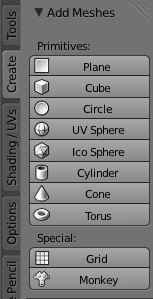
\includegraphics[scale=0.5]{spinehead1.png}
        \end{figure}

\item   Rename the sphere. Double-click the entry box below to change the default name to 'SpineHead'.
        \begin{figure}[H]
        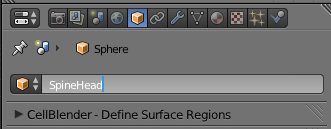
\includegraphics[scale=0.5]{spinehead2.png}
        \end{figure}

    \item   Change view to see the sphere from the 'Front' view. (shortcut: 1 on numpad). Note, it is \textbf{extremely} important that the user be in orthographic mode (shortcut: 5 on numpad) during Blender work.

\item   Deselect the sphere (shortcut: a) and make it transparent (shortcut: z)

\item   Select the vertices to be removed. First, switch from 'Object Mode' to 'Edit Mode'. Ensure that 'Edge select' is enabled. Then use box select (shortcut: b) to capture only the faces that make up the top half of the sphere. Delete these faces (shortcut: x) and select the 'Faces' option in the delete menu.
        \begin{figure}[H]
        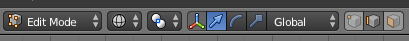
\includegraphics[scale=0.5]{spinehead3.png}
        \end{figure}

\item   Close the opening. Select the topmost vertices (remaining in 'Edge select' mode) using box select (shortcut: b). Then, extrude (shortcut: e) and click 'Edges Only' under 'Extrude' in 'Mesh Tools'.        
        \begin{figure}[H]
        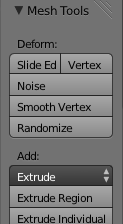
\includegraphics[scale=0.5]{spinehead4.png}
        \end{figure}
        Set the extrude distance by pressing 0 and Enter to confirm. Scale the extrusion by pressing s, 0 and Enter to confirm. Select 'Remove Doubles' under 'Mesh Tools' to remove the duplicated vertices and reconnect the triangles. Blender should note that you remove 15 vertices as a result.
        \begin{figure}[H]
        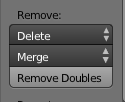
\includegraphics[scale=0.5]{spinehead5.png}
        \end{figure}
        The object should now be closed by a flat top.

\end{enumerate}

\subsection{Creating a presynaptic bouton}

\begin{enumerate}
    \item   Duplicate the \textit{spine.blend} file as \textit{bouton.blend}. in \textit{bouton.blend} deselect all (shortcut: a).
    
\item   Duplicate the spine head and rotate. First, switch to 'Front' view (shortcut: 1 on numpad). Duplicate (shortcut: Shift-d, Enter) and rotate 180 degrees (shortcut: r, 180, Enter). To separate the selection of the spine heads, press p and click 'Selection'.

\item   Rename the item. Switch to 'Object Mode' (shortcut: Tab) and edit the name field to 'PresynapticBouton'.
        \begin{figure}[H]
        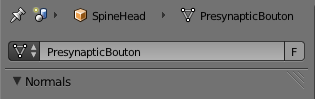
\includegraphics[scale=0.5]{bouton1.png}
        \end{figure}

\item   Shift and scale the bouton. Grab the object (shortcut: g), constrain movement to the z-axis (shortcut: z) and type 0.023, \textit{Enter} to move the object. 
\end{enumerate}

\subsection{Adding Axonal and Dendritic Extensions}

\begin{enumerate}

\item   Enter 'Edit Mode' (shortcut: Tab), and switch view to front (shortcut: 1 on numpad)

\item   Zoom in on the top of the vertex. Select the vertex by right-clicking on it, ensuring that 'Vertex mode' selection is enabled. Perform two 'Select More' operations (shortcut: Control-Plus on numpad) until two rings are highlighted. Press x, select 'Faces' on the menu, \textit{Enter} to confirm. Press b and select the vertices on the top edge using 'Box select'. Press e, click on 'Edges Only' in 'Tools' (left pane), then type z, 3.0, \textit{Enter}. This should produce an axon on the presynaptic bouton.

\item   Select the spine head. Hit \textit{Tab} to enter 'Object Mode' and right click the spine head (the bottom half-sphere) to select it. \textit{Tab} back into 'Edit Mode'

\item   Create a cylindrical spine on the spine head. As in the earlier step, select the bottom vertex, perform two 'Select More' operations, press x and select 'Faces' on the 'Erase' menu. Hit b and select the vertices that line the hole in the bottom. Press e, select 'Edges Only' in 'Tools', press z, type -2.0, \textit{Enter}. 

\end{enumerate}

\subsection{Add Synaptic Vesicles with Regions for Calcium Binding}

\begin{enumerate}
\item   Create the first vesicle. First, ensure that the object is at the origin by moving it if necessary (shortcut: g). Move the cursor to the origin (shortcut: \textit{Shift}-c). Ensure that 'Object Mode' is enabled. Under the 'Create' tab at left, select Ico-Sphere. A pane appears at lower left - change the default settings to 1 subdivision and a size of 0.023. A small sphere should appear at the origin.

\item   It is necessary to rotate the vesicle. With the sphere selected, press r, x, 90, \textit{Enter} to align the sphere with the x-axis. Enter the 'Outliner' pane at the top right, and edit the name of the sphere to 'Vesicle\_1'.

\item   Define the calcium binding region. With the vesicle still selected, change to 'Edit Mode' (shortcut: \textit{Tab}) and triangulate the faces (shortcut: \textit{Control-t}). First, select the 'Define Surface Region' tab which is under the 'Object' tab. Add a new region and name it 'vesicle\_1\_surf' (for the surface region of the vesicle). With the vesicle selected, click 'Assign'. We must now add the vesicle to the list of mesh objects to be included in the simulation. Under the 'Scene' tab, select 'Model Objects' and add the vesicle to this list. A green tick should appear.
        \begin{figure}[H]
        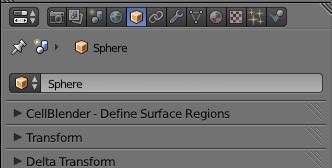
\includegraphics[scale=0.5]{vesicle1.png}
        \end{figure}

\item   Move the vesicle. Tab into 'Object Mode', press g to grab the vesicle, type x, -0.108 \textit{Enter} to move the vesicle along the x-axis. Hit g, 0.105, \textit{Enter} to move it 0.105 units along the z-axis. 

\item   Duplicate the vesicle. Hit \textit{Shift}-d, g, 0.216, \textit{Enter} to move the vesicle the appropriate distance. This vesicle should appear as a new object under the 'Scene' pane - rename this vesicle to 'Vesicle\_2' and repeat the steps for defining the surface region, this time naming it 'vesicle\_2\_surf'.
        \begin{figure}[H]
        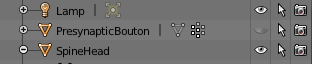
\includegraphics[scale=0.5]{vesicle3.png}
        \end{figure}


\end{enumerate}

\subsection{Defining region for voltage-gated calcium channels (VGCC)}

\begin{enumerate}
\item   Clip the existing mesh objects. Use \textit{Alt-b} to draw a box around the presynaptic terminal and the vesicles. This will only show those items and hide the rest of the model. It is helpful to switch into 'Edit Mode', turn on wireframe (shortcut: z) and switch camera view to side (shortcut: 1,3 on numpad).
    
\item   Switch to overhead view. Hit 7 on the numpad to look down from above on the vesicles. 

\item   Create the regions. We will create two small planes under each vesicle which will represent the VGCCs. Use the 'Plane' tool under 'Create' to define a plane. Adjust the settings using the 'Add Plane' pane at bottom left to position it underneath the vesicle. Duplicate it and copy it over to the other vesicle in the same fashion used to duplicate the vesicle. 

\item Group the regions. With both panes selected, use \textit{Ctrl-p} to merge the regions as one.

\item   Assign the selected regions. In the bottom right pane under 'Objects', go to 'Define Surface Region', and label it 'vgcc\_region'. We want this region to be an object in its own right for later selection and editing. With the region selected, press p and hit 'Selection'. Rename the object created to 'VGCC' in the top right pane. Remove the clipping box by pressing \textit{Alt-b}.
\end{enumerate}

\subsection{Defining region for postsynaptic receptors}

\begin{enumerate}
\item   Hide the presynaptic bouton and the VGCC's. Click the eye button on the top right pane for the appropriate objects.

\item   Define the postsynaptic receptor region. Right click on the postsynaptic dendrite and select the top face using the bounding box (shortcut: b). Use two 'Select Less' operations (shortcut: Control - minus on numpad) to deselect two outer rings. 

\item   Assign region. Under 'Objects' go to 'Define Surface Region' and label the receptor as 'postsynaptic\_receptor'. In CellBlender, this region will now accessed as 'SpineHead[postsynaptic\_receptor]'. Press \textit{Control - t} to triangulate the faces, and then add it under 'Scene' in 'Model Objects'.

\end{enumerate}

\subsection{Adding Objects to CellBlender}
The following objects should be under 'Model Objects':

\begin{enumerate}
    \item PresynapticBouton
    \item SpineHead
    \item VGCC
    \item Vesicle\_1
    \item Vesicle\_2
\end{enumerate}

If not, simply select the model item, triangulate (shortcut: \textit{Control}-t) and then with the item still selected add it under 'Model Objects'. This allows MCell to recognise the Blender object as part of the simulation.

\subsection{Editing Model Object Appearance} % (fold)
\label{sub:Editing Model Object Appearance}

% subsection Editing Model Object Appearance (end)
Here are some steps which will improve the visualisation of our setup.

First, we want to make the presynaptic bouton semi-transparent so that we can see what is occuring inside the synapse. Under the 'Material' tab (look for the little red ball) create a new material by hitting the plus sign. Click the drag-down box and change the mode from 'Object' to 'Data'. Select the presynaptic bouton, enter 'Edit Mode' and assign the new material to the selected surface. Under 'Transparency', change the alpha level to 0.3. Exit 'Edit Mode'; the surface should be semi-transparent. If it is not, then under 'Objects', go to 'Display' and turn on 'Transparency'.

    \begin{figure}[H]
        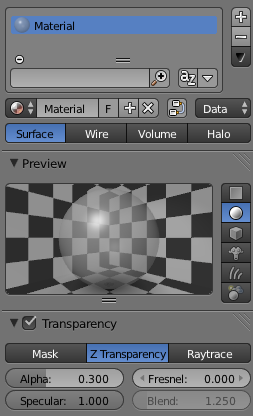
\includegraphics[scale=0.5]{settings3.png}
    \end{figure}

CellBlender will assign each molecule a certain colour automatically. If you want to change this, then go to the 'Outliner' (top right pane listing all the objects in the scene) and under 'molecules' go to the molecule of your choice. Click the small '+' to expand. For a molecule named 'a', you will see 'mol\_a\_pos' and 'mol\_a\_shaape'. Click on shape, and then navigate to 'Materials' (the little red ball) to change its colour.


\subsection{Making Copies of the Model}
At this stage, we have completed the model geometry - all the Blender objects have been set up for simulation. Make a copy of the file  (File -> Save As) by saving it under another name. One copy will be used in the next section (Phase I Simulation) while the other will be used in the section after (Phase II Simulation).

Phase I deals with the diffusion of calcium, the triggering of the SNAREpin mechanisms, and the fusion times of the vesicles, while Phase II deals with the release of neurotransmitter and the binding to receptors.

\section{Simulation using the CellBlender Interface - Phase I}

In this section, we simulate the fusion of the vesicles via a SNAREpin activation mechanism. We record the release times by creating tags for the 'fused' vesicles. Through an external Python script we record these times in preparation for the next phase.


\subsection{Specification of Molecules}
The following molecules will need to be added to our simulation under 'Scene' in 'Define Molecules'. The format is name of molecule, type of molecule, and diffusion constant.

\begin{enumerate}
    \item Ca, Volume, 1e-6
    \item VGCC\_C, Surface, 0
    \item VGCC\_O, Surface, 0
    \item CaBS, Surface, 0
    \item CaBS\_Ca, Surface, 0
    \item TAG, Surface, 0
\end{enumerate}

\subsection{Define Reactions between Molecules}
Given a set of molecules, we must define the interactions that occur when molecules meet. Under 'Define Reactions', enter the following (consists of reactants, products, and forward rate constant):

\begin{enumerate}
    \item VGCC\_C' $\to$ VGCC\_O', 5e5
    \item VGCC\_O' $\to$ VGCC\_C', 500
    \item VGCC\_O' $\to$ VGCC\_O' + Ca', 1e3
    \item Ca' + CaBS' $\to$ CaBS\_Ca', 1e7
    \item CaBS\_Ca' + Ca' $\to$ TAG', 1e9
\end{enumerate}

The apostrophes are used to indicate to CellBlender the geometry at which the reaction occurs.


\subsection{Adding Molecules to Regions}
We only want the closed VGCC's and the calcium binding sites 'CaBS' to be present when the model is initialised. All other molecules will be generated by the reactions during simulation. The following items will be added under 'Molecule Release/Placement'. 

Create a site called 'vgcc\_rel'. This will be situated on the surface named 'VGCC[vgcc\_reg]', and will represent the calcium channels. Enter the following settings.
    \begin{figure}[H]
        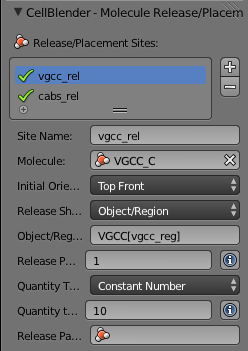
\includegraphics[scale=0.5]{settings1.png}
    \end{figure}


Similarly, create a site called 'cabs\_rel\_1'. This will be situated on the 'Vesicle\_1[vesicle\_1\_surf]' and will represent the calcium release sites. Enter the following settings.
    \begin{figure}[H]
        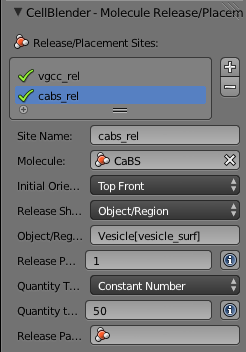
\includegraphics[scale=0.5]{settings2.png}
    \end{figure}

Repeat again for 'cabs\_rel\_2', with identical settings.

\subsection{Modifying and Defining Surface Classes}
It may be desirable to define surface classes so that the surfaces in the model mimic real neuron surface structures better. 

We can create surface classes under the 'Define Surface Classes' option. Create a surface class and add a property. The properties have three attributes - molecule, orientation, and type. 

For this section, we will create a surface class called 'ca\_absorb'. It will affect the Ca molecule, have Top/Front orientation, and have the type 'Absorb'. We then assign under 'Modify Surface Regions' this surface class to the presynaptic bouton - 'PresynapticBouton[presynaptic\_shell]'.
 
Once the above instructions are complete, skip ahead and complete all the instructions under 'Preparing for Simulation' . Then, save the file and quit.

\section{Simulating using the CellBlender Interface - Phase II}
In this phase, we simulate the timed release of neurotransmitter molecules and their subsequent interaction with the receptor region on the spine head. The release times are obtained from the first phase of our simulation.

Complete the following instructions in the second copy of the Blender geometry.
\subsection{Glial Cell Proxy}
In the postsynaptic phase, neurotransmitter molecules will be dumped into the synaptic cleft and then will either contact a receptor or diffuse out of the cleft. In reality, these neurotransmitter molecules will be collected by glial cells and returned to neuron.

We can simulate this action by defining a cylinder around the whole synapse. Centre the cursor (shortcut: \textit{Crtl}-b) and then create the cylinder. At the 'Add Cylinder' pane at bottom left, leave the radius at the default of 1.0, but ensure that for 'Cap Fill Type' the option 'None' is selected. Enter 'Edit Mode', select the whole cylinder, and then triangulate the object (shortcut: \textit{Crtl}-t). Add the cylinder under 'Model Objects'. Define a surface region called 'surface' under 'Add Surface Regions'. Finally, name the cylinder 'GlialCells'. 


\subsection{Specification of Molecules}
We want to add the following molecules to our simulation. The instruction format is once again molecule, molecule type, and rate constant.

\begin{enumerate}
    \item NT, Volume, 5.3e-6
    \item LGIC\_C, Surface, 0
    \item LGIC\_O, Surface, 0
\end{enumerate} 

\subsection{Define Reactions between Molecules}
We want to specify interactions between our molecules. There is only one relevant reaction in this case.

\begin{enumerate}
    \item NT' + LGIC\_C' $\to$ LGIC\_O', 4.6e6
\end{enumerate}

\subsection{Modifying and Defining Surface Classes}
We want to create surface classes called 'nt\_absorb' and 'nt\_reflect'. They both affect the NT molecule, and have the types 'Absorb' and 'Reflective' respectively. We assign 'nt\_absorb' to a single region - GlialCells[surface]. We assign 'nt\_reflect' to two regions - PresynapticBouton[presynaptic\_membrane] and SpineHead[receptor\_region].

\section{Preparing for Simulation}
The instructions for this section are to be completed for both parts of the simulation.

Under 'Model Initialization', set the iterations to 10000 and the time step to 1e-6 (the amount of simulation time that passes between frames).

Under 'Reaction Output Settings', add an item for each molecule (should end up with 5 counts altogether). This setting will keep track of the number of molecules of each type currently existing in the model environment.

Ensure that the data is saved before continuing.

Refer to the IPython Notebook which contains the remainder of the instructions. These instructions are also integrated with scripts which perform backend tasks.

\section{Rendering}
Once the simulation is complete, the reader may wish to render their results to produce an animation of their model.

First, orientate the viewport to the view which is to be rendered.

Then, add a camera (Add $\to$ Camera). Right-click it to select, and then select the 'Align Active Camera to View' option (shortcut: Crtl Atl Numpad 0).

Next, click on the 'Render' pane. The following settings are the ones used to generate the animation files; however, the appropriate settings will depend on the computer used to generate the render. For example, it is not necessary to render all the frames - a subset can be selected if so desired.

\begin{figure}[H]
    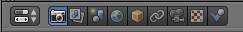
\includegraphics[scale=0.5]{render1.png}
\end{figure}

\begin{figure}[H]
    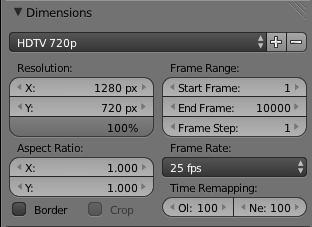
\includegraphics[scale=0.5]{render2.png}
\end{figure}

Scroll down to 'Output' and select an appropriate folder. Scroll up to the top and hit 'Animation; then wait. This will take a while. 

\section{Troubleshooting}
\marginlabel{Simulation doesn't run} First, under 'Run Simulation' ensure that both output and error logs are being sent to file. Inspection of the error log in particular should reveal the cause of the issue. The most common error is a failure to properly assign a surface region to a Blender object - ensure that all regions are properly assigned before commencing a simulation run.

    \begin{figure}[H]
        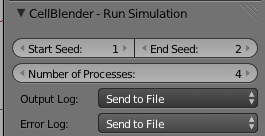
\includegraphics[scale=0.5]{trouble1.png}
    \end{figure}

\end{document}
